\documentclass[12pt,letterpaper]{article}
\usepackage{graphicx,textcomp}
\usepackage{natbib}
\usepackage{setspace}
\usepackage{fullpage}
\usepackage{color}
\usepackage[reqno]{amsmath}
\usepackage{amsthm}
\usepackage{fancyvrb}
\usepackage{amssymb,enumerate}
\usepackage[all]{xy}
\usepackage{endnotes}
\usepackage{lscape}
\newtheorem{com}{Comment}
\usepackage{float}
\usepackage{hyperref}
\newtheorem{lem} {Lemma}
\newtheorem{prop}{Proposition}
\newtheorem{thm}{Theorem}
\newtheorem{defn}{Definition}
\newtheorem{cor}{Corollary}
\newtheorem{obs}{Observation}
\usepackage[compact]{titlesec}
\usepackage{dcolumn}
\usepackage{tikz}
\usetikzlibrary{arrows}
\usepackage{multirow}
\usepackage{xcolor}
\newcolumntype{.}{D{.}{.}{-1}}
\newcolumntype{d}[1]{D{.}{.}{#1}}
\definecolor{light-gray}{gray}{0.65}
\usepackage{url}
\usepackage{listings}
\usepackage{color}
\usepackage{listings}


\definecolor{codegreen}{rgb}{0,0.6,0}
\definecolor{codegray}{rgb}{0.5,0.5,0.5}
\definecolor{codepurple}{rgb}{0.58,0,0.82}
\definecolor{backcolour}{rgb}{0.95,0.95,0.92}

\lstdefinestyle{mystyle}{
	backgroundcolor=\color{backcolour},   
	commentstyle=\color{codegreen},
	keywordstyle=\color{magenta},
	numberstyle=\tiny\color{codegray},
	stringstyle=\color{codepurple},
	basicstyle=\footnotesize,
	breakatwhitespace=false,         
	breaklines=true,                 
	captionpos=b,                    
	keepspaces=true,                 
	numbers=left,                    
	numbersep=5pt,                  
	showspaces=false,                
	showstringspaces=false,
	showtabs=false,                  
	tabsize=2
}
\lstset{style=mystyle}
\newcommand{\Sref}[1]{Section~\ref{#1}}
\newtheorem{hyp}{Hypothesis}

\title{Problem Set 1}
\date{Due: October 8, 2026}
\author{Nianci You Student Number:26338956}

\begin{document}
	\maketitle
	
	\section*{Instructions}
	\begin{itemize}
	\item Please show your work! You may lose points by simply writing in the answer. If the problem requires you to execute commands in \texttt{R}, please include the code you used to get your answers. Please also include the \texttt{.R} file that contains your code. If you are not sure if work needs to be shown for a particular problem, please ask.
\item Your homework should be submitted electronically on GitHub.
\item This problem set is due before 23:59 on Thursday October 8, 2026. No late assignments will be accepted.
	\end{itemize}
	
	\vspace{1cm}
	\section*{Question 1: Education}

A school counselor was curious about the average of IQ of the students in her school and took a random sample of 25 students' IQ scores. The following is the data set:\\
\vspace{.5cm}

\lstinputlisting[language=R, firstline=40, lastline=40]{PS01.R}  


\vspace{1cm}

\begin{enumerate}
	\item Find a 90\% confidence interval for the average student IQ in the school (As a hint, you first need the mean and SD to create a CI):\\
	
	  \lstinputlisting[language=R, firstline=42, lastline=56]{PS01.R} 
	  
	  \noindent The sample has a mean IQ of 98.44 and a sample standard deviation of 13.09. The standard error is $\displaystyle \frac{13.09}{\sqrt25}=2.62$, and the critical value for the 90\% CI is 1.71. Therefore, the 90\% CI for the average student IQ in the school is [93.96 and 102.91]. \\ \\
	  

	
	\item Next, the school counselor was curious  whether  the average student IQ in her school is higher than the average IQ score (100) among all the schools in the country.\\ 
	\noindent Using the same sample, conduct the appropriate hypothesis test with $\alpha=0.05$.
	

	
	\lstinputlisting[language=R, firstline=64, lastline=68]{PS01.R}
	   
	   
	   \noindent  H0: the average student IQ in the school is equal to 100 
	   
	   H1: the average student IQ in the school is larger than 100 
	   
	   A one-side one sample t test is used to test H1 and H0. The result of the t-test is shown below:
	   
	   
% Error: Unrecognized object type. 

% Error: Unrecognized object type. 

% Error: Unrecognized object type. 

% Error: Unrecognized object type. 

% Error: Unrecognized object type. 

% Table created by stargazer v.5.2.3 by Marek Hlavac, Social Policy Institute. E-mail: marek.hlavac at gmail.com
% Date and time: Mon, Oct 05, 2026 - 12:11:16
\begin{table}[!htbp] \centering 
  \caption{Result of T Test} 
  \label{} 
\begin{tabular}{@{\extracolsep{5pt}} cccccccc} 
\\[-1.8ex]\hline 
\hline \\[-1.8ex] 
estimate & statistic & p.value & parameter & conf.low & conf.high & method & alternative \\ 
\hline \\[-1.8ex] 
$98.440$ & $$-$0.596$ & $0.722$ & $24$ & $93.960$ & $Inf$ & One Sample t-test & greater \\ 
\hline \\[-1.8ex] 
\end{tabular} 
\end{table}  

	   
	   \noindent The t test statistic is -0.596, the p value is 0.722. As the p value is greater than 0.05, we fail to reject H0. This means that there is no sufficient evidence to prove that the average student IQ score in this school is higher than the average IQ score among all the schools in the country.
	   
	  
	
\end{enumerate}

\newpage

	\section*{Question 2: Political Economy}

\noindent Researchers are curious about what affects the amount of money communities spend on addressing homelessness. The following variables constitute our data set about social welfare expenditures in the USA. \\
\vspace{.5cm}


\begin{tabular}{r|l}
	\texttt{State} &\emph{50 states in US} \\
	\texttt{Y} & \emph{per capita expenditure on shelters/housing assistance in state}\\
	\texttt{X1} &\emph{per capita personal income in state} \\
	\texttt{X2} &  \emph{Number of residents per 100,000 that are "financially insecure" in state}\\
	\texttt{X3} &  \emph{Number of people per thousand residing in urban areas in state} \\
	\texttt{Region} &  \emph{1=Northeast, 2= North Central, 3= South, 4=West} \\
\end{tabular}

\vspace{.5cm}
\noindent Explore the \texttt{expenditure} data set and import data into \texttt{R}.
\vspace{.5cm}
\lstinputlisting[language=R, firstline=91, lastline=92]{PS01.R}  
\vspace{.5cm}
\begin{itemize}

\item
Please plot the relationships among \emph{Y}, \emph{X1}, \emph{X2}, and \emph{X3}? What are the correlations among them (you just need to describe the graph and the relationships among them)?
    \vspace{20cm}
    
    \lstinputlisting[language=R, firstline=94, lastline=103]{PS01.R}  

   \begin{figure}[h!]\centering
   	\caption{\footnotesize Scatterplot Matrix of Y, X1, X2 and X3}
   	\label{fig:plot_1}
   	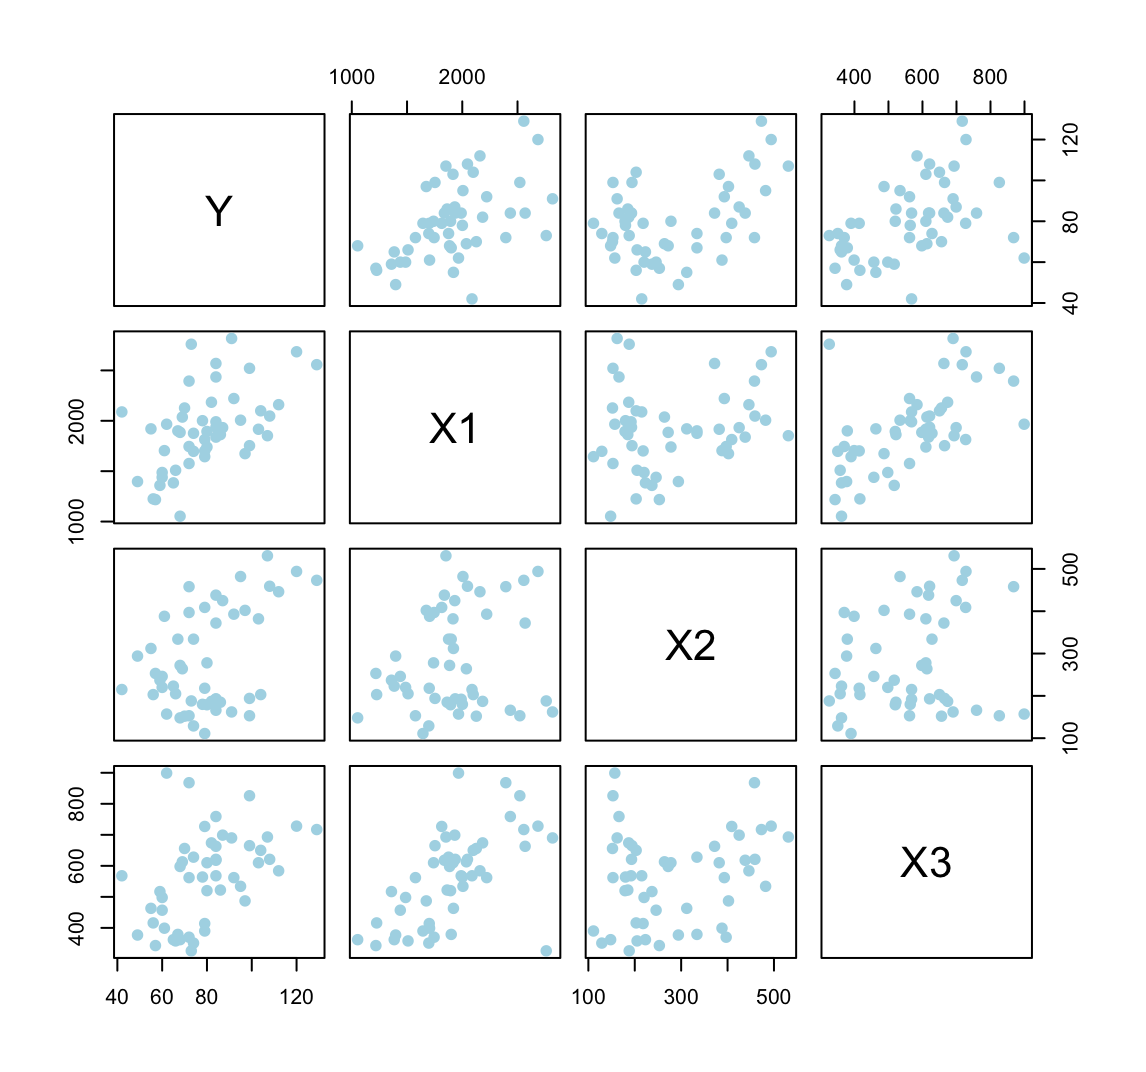
\includegraphics[width=.75\textwidth]{2.1.png}
   \end{figure}
   
  \noindent The scatterplot matrix shows the relationships among per capita housing assistance expenditure(Y), per capita personal income(X1), financial insecurity(X2), and urban residence(X3). \\
  
  All pairwise correlations are positive. The clearest upward pattern is between X1 and X3, followed by Y and X1. Y also shows positive correlations with X2 and X3, although the points are more dispersed. The relationships of X1 and X2 and of X2 and X3 are weaker. \\ \\
  
  
% Table created by stargazer v.5.2.3 by Marek Hlavac, Social Policy Institute. E-mail: marek.hlavac at gmail.com
% Date and time: Tue, Oct 06, 2026 - 10:57:42
\begin{table}[!htbp] \centering 
  \caption{Pearsn Correlation Coefficient Matrix} 
  \label{} 
\begin{tabular}{@{\extracolsep{5pt}} cccc} 
\\[-1.8ex]\hline 
\hline \\[-1.8ex] 
Y & X1 & X2 & X3 \\ 
\hline \\[-1.8ex] 
$1$ & $0.532$ & $0.448$ & $0.464$ \\ 
$0.532$ & $1$ & $0.206$ & $0.595$ \\ 
$0.448$ & $0.206$ & $1$ & $0.221$ \\ 
$0.464$ & $0.595$ & $0.221$ & $1$ \\ 
\hline \\[-1.8ex] 
\end{tabular} 
\end{table}  

  
  \vspace{.5cm}
  
  \noindent The result of the Pearson correlation coefficient matrix quantifies the strength of relationships observed in the scatterplot matrix, showing more specific results. The Pearson coefficient matrix supports the visual patterns obsered in the matrix. The Pearson coefficient is the largest between X1 and X3( r = 0.595), followed by the coefficient between Y and X1 (r = 0.532). The coefficient between X1 and X2 is the weakest (r = 0.206). \\ \\

\item
Please plot the relationship between \emph{Y} and \emph{Region}? On average, which region has the highest per capita expenditure on housing assistance?
\vspace{18cm}

 \lstinputlisting[language=R, firstline=127, lastline=136]{PS01.R}  

\begin{figure}[h!]\centering
	\caption{\footnotesize Per Capita Housing Expenditure by Region}
	\label{fig:plot_2}
	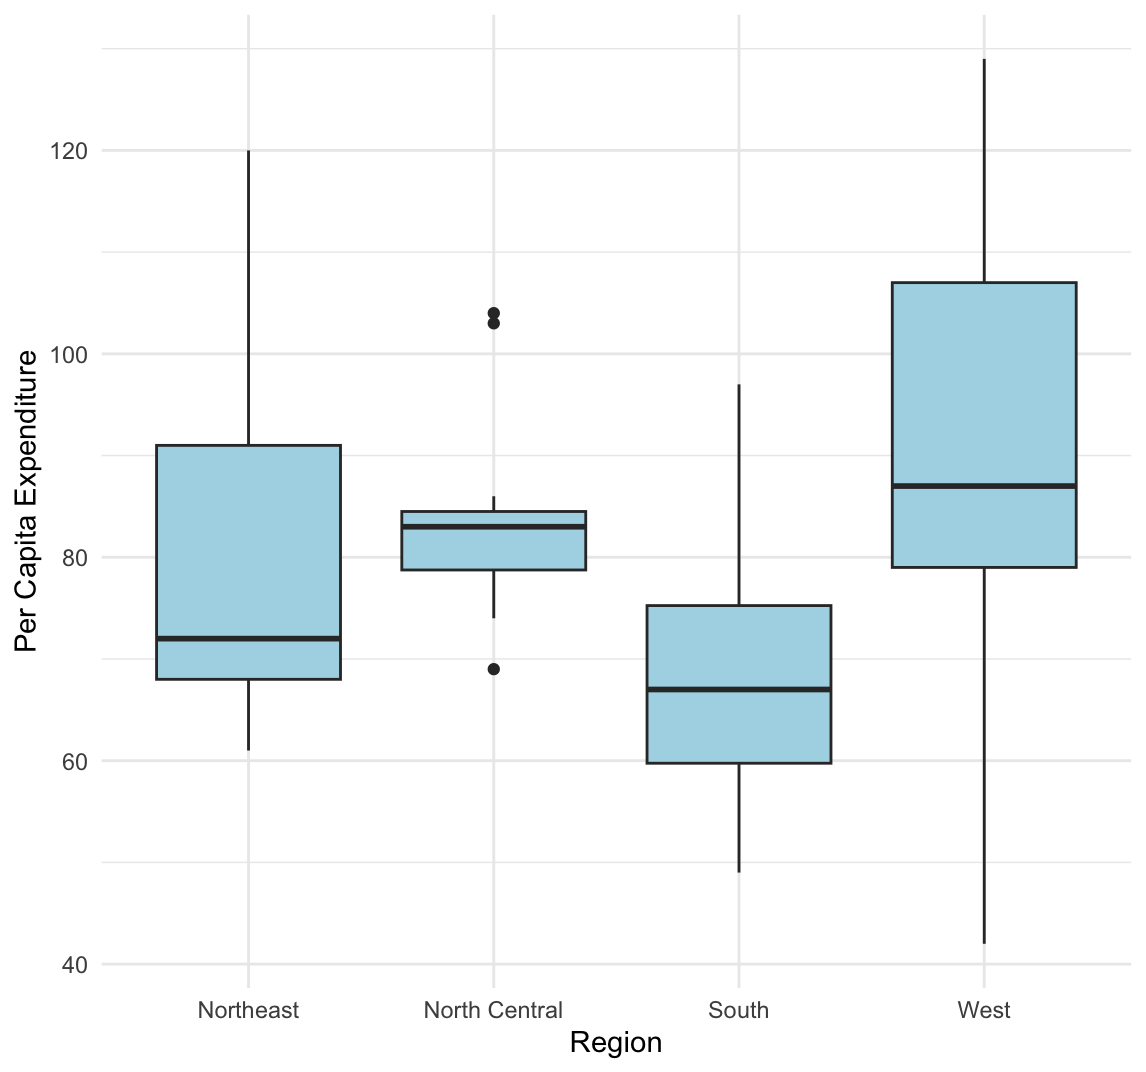
\includegraphics[width=.75\textwidth]{2.2.png}
\end{figure}

\noindent The boxplot compares the distribution of per capita housing assistance expenditure across the four regions. The west has the highest median, while the south has the lowest. Therefore, the west spends the most on housing assistance per capita on average. \\ \\

\item
Please plot the relationship between \emph{Y} and \emph{X1}? Describe this graph and the relationship. Reproduce the above graph including one more variable \emph{Region} and display different regions with different types of symbols and colors.

\lstinputlisting[language=R, firstline=144, lastline=162]{PS01.R}  
\vspace{20cm}

    \begin{figure}[h!]\centering
    	\caption{\footnotesize Relationship between expenditure on housing assistance(Y) and personal income(X1)}
    	\label{fig:plot_3}
    	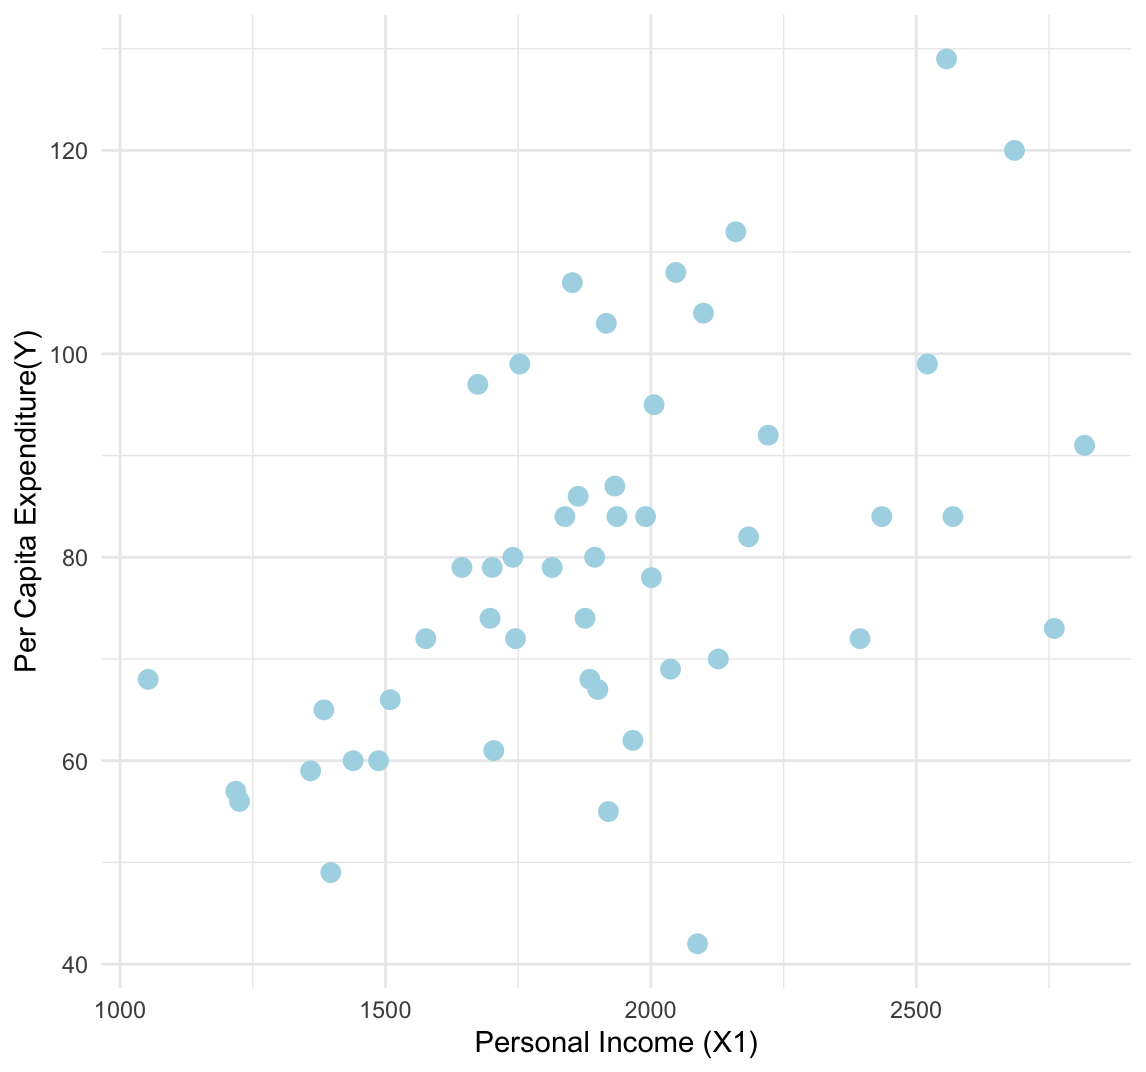
\includegraphics[width=.75\textwidth]{2.3.1.png}
    \end{figure} 
    
     \noindent The scatter plot shows the relationship between per capita personal income(X1) and per capita housing assistance expenditure (Y). When personal income increases, the expenditure on housing assistance also tend to increase.
     
     
     \vspace{20cm}
     
      \begin{figure}[h!]\centering
     	\caption{\footnotesize Per Capita Housing Assistance Expenditure and Personal Income By Region}
     	\label{fig:plot_4}
     	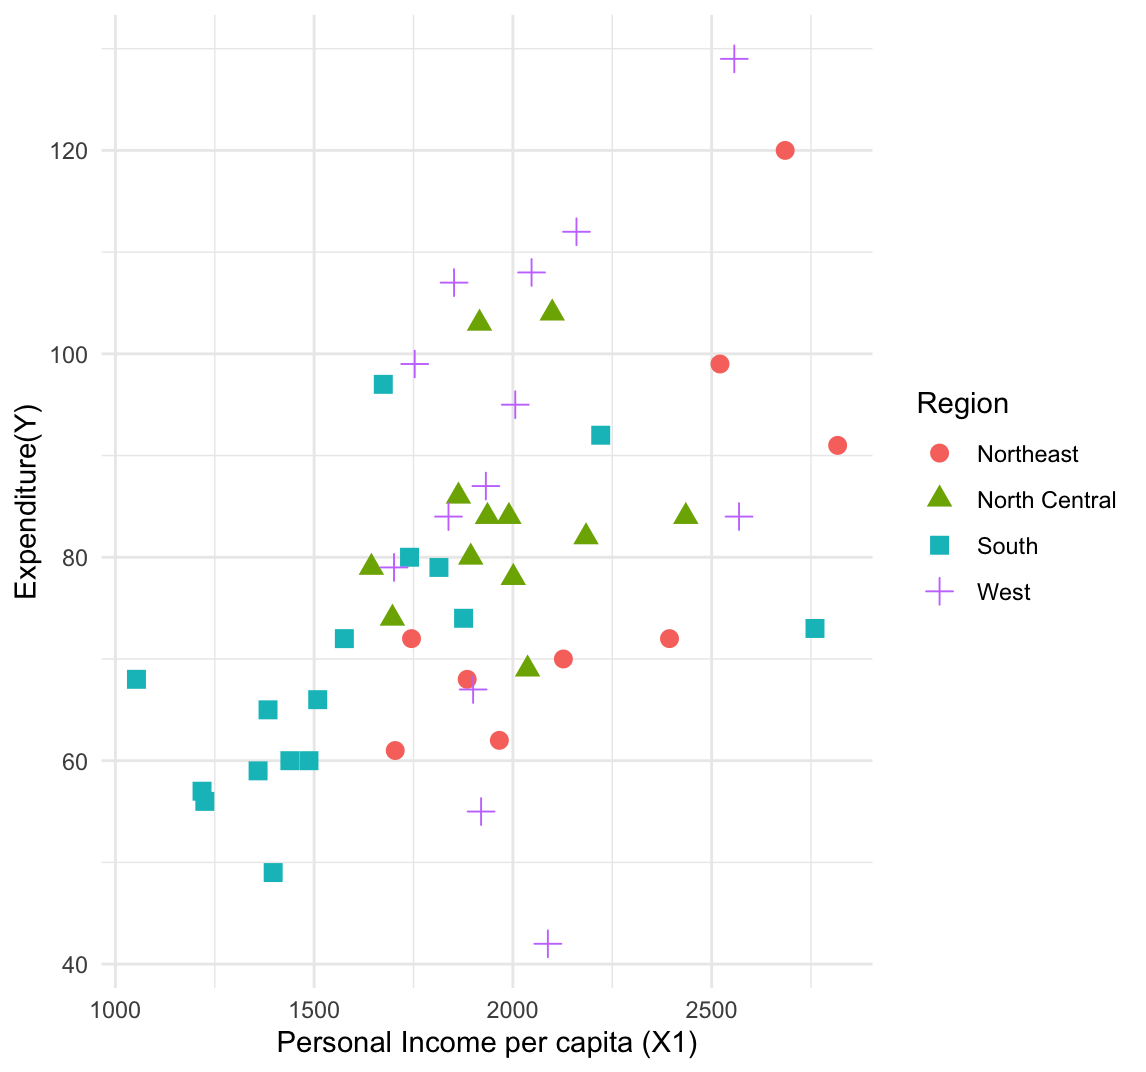
\includegraphics[width=.75\textwidth]{2.3.2.png}
     \end{figure} 
     
     
     \noindent The second scatterplot distinguishes the four regions using four different symbols and colours. The overall positive association remains the same, while the regional distributions differ. 
     
     The northeast shows a broad spread in both income and expenditure. The north central region is more tightly clustered, particularly around intermediate income and expenditure levels. Most states in the south region lies toward the lower income and expenditure level of the plot, although some have higher values. The west region shows a wide range of expenditure, including very high and or intermediate levels of personal income.
     
   
     
    
\end{itemize}

    

\end{document}
